\chapter*{Übung 4}

\section*{Aufgabe 8}

Erinnerung: $\dot{x}(t) = \msimplediff{x(t)}{t}$ und $\ddot{x}(t) = \frac{\mathrm{d}^2 x(t)}{\mathrm{d} t^2}$.

Zu lösende Gleichung:
\[
	\ddot{x}(t) = -\frac{k}{m} x(t)
	\text{.}
\]

Ansatz: $x(t) = c_\lambda e^{\lambda t}$; also $\dot{x}(t) = \lambda c_\lambda e^{\lambda t}$ und $\ddot{x}(t) = \lambda^2 c_\lambda e^{\lambda t}$. Das in die zu lösende Gleichung einsetzen:
\[
	\lambda^2 c_\lambda c^{\lambda t} = -\frac{k}{m} c_\lambda e^{\lambda t}
	\quad \Longleftrightarrow \quad
	\lambda^2 = -\frac{k}{m}
	\quad \Longrightarrow \quad
	\lambda = \pm i \sqrt{\frac{k}{m}}
	\text{.}
\]

Die allgemeine Lösung lautet also: $x(t) = c_1 e^{it \sqrt{k / m}} + c_2 e^{-it \sqrt{k / m}}$ und die Ableitung davn ist: $\dot{x}(t) = \sqrt{\frac{k}{m}} \left( c_1 e^{it \sqrt{k / m}} - c_2 e^{-it \sqrt{k / m}} \right)$.

Nun sollen die Konstanten $c_1$ und $c_2$ bestimmt werden. Dazu die Anfangsbedingungen einsetzen:
\begin{align*}
	x_0 &\overset{!}{=} x(t = 0) = c_1 + c_2,	 \\
	v_0 &\overset{!}{=} \dot{x}(t = 0) = i \sqrt{\frac{k}{m}} (c_1 - c_2)
	\text{.}
\end{align*}
Das führt auf $c_1 = \frac{1}{2} \left( x_0 + \frac{1}{i} \sqrt{\frac{m}{k}} v_0 \right)$ und $c_2 = \frac{1}{2} \left( x_0 - \frac{1}{i} \sqrt{\frac{m}{k}} v_0 \right)$. Eingesetzt ergibt das die Lösung
\[
	x(t) = \frac{1}{2} x_0 \left( e^{it \sqrt{k / m}} + e^{-it \sqrt{k / m}} \right)
	+ \frac{1}{2i} \sqrt{\frac{m}{k}} v_0 \left( e^{it \sqrt{k / m}} - e^{-it \sqrt{k / m}} \right)
	\text{.}
\]

Um den Term weiter zu vereinfachen, verwende $\frac{k}{m} = \omega^2$. Das führt auf auf die vereinfachte Lösung
\[
	x(t) = x_0 \cos(\omega t) + \frac{v_0}{\omega} \sin(\omega t)
	\text{.}
\]

Zuletzt berechnen wir die Energie, wobei $\dot{x}(t) = -x_0 \omega \sin(\omega t) + v_0 \omega \cos(\omega t)$:
\begin{align*}
	E &= T + V = \frac{1}{2} m \dot{x}^2 + \frac{1}{2} k x^2	 = \frac{1}{2} m \left( \dot{x}^2(t) + \omega^2 x^2(t) \right) \\
	&= \dots = \frac{1}{2} m \left( v_0^2 + \omega^2 x_0^2 \right) = \frac{1}{2} m v_0^2 + \frac{1}{2} k x_0^2
	\text{.}
\end{align*}

\section*{Aufgabe 9}
Siehe Abbildung \ref{fig:ueb4_aufgabe9} für eine Skizze mit den Variablen.

\begin{figure}[h]
	\centering
	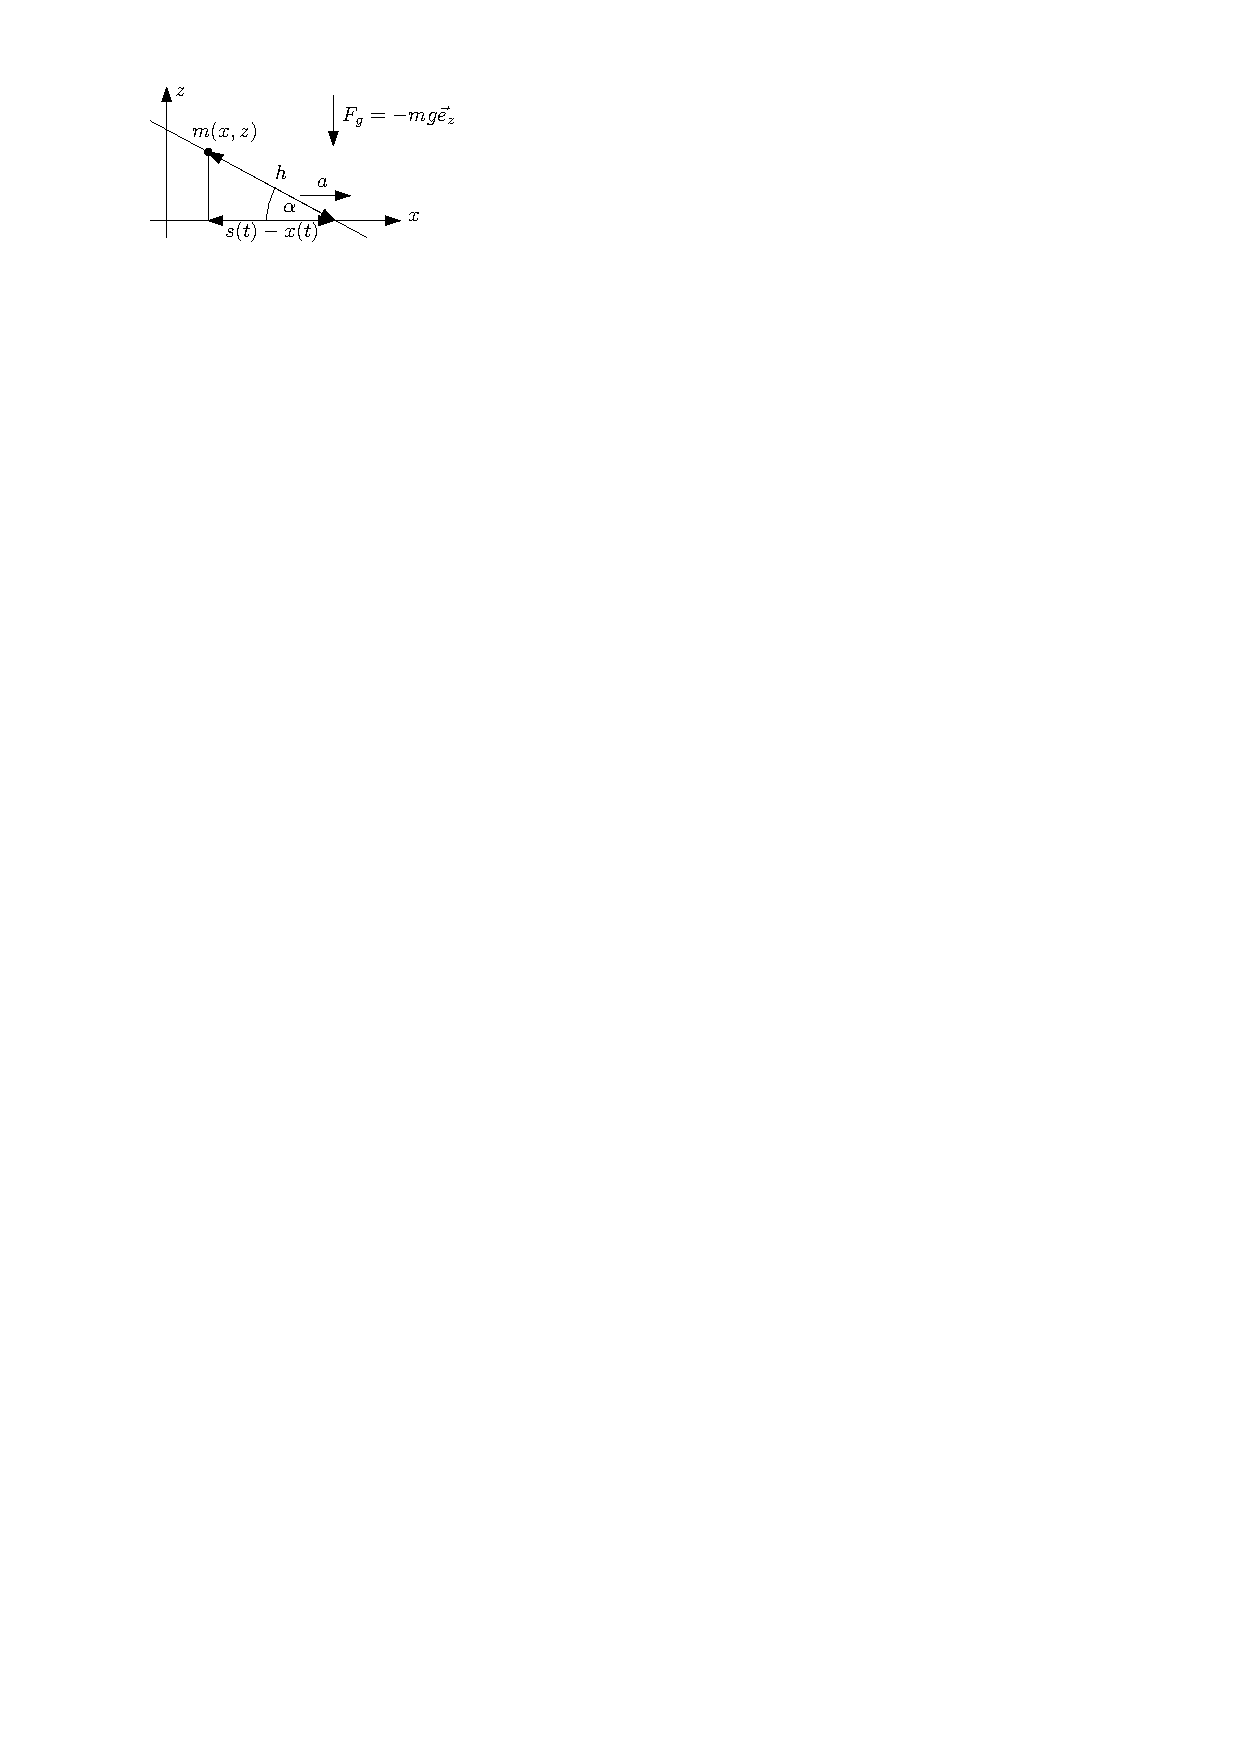
\includegraphics[scale=1.5]{figures/ueb4/aufgabe9}
	\caption{Skizze für die Variablen von Aufgabe 9.}
	\label{fig:ueb4_aufgabe9}
\end{figure}

Es gilt $\sin \alpha = \frac{z(t)}{h}$ und $\cos \alpha = \frac{s(t) - x(t)}{h}$, also
\[
	\frac{z(t)}{\sin \alpha} = \frac{s(t) - x(t)}{\cos \alpha}
	\quad \Longleftrightarrow \quad 
	z(t) \cos(\alpha) = (s(t) - x(t)) \sin \alpha
	\text{.}
\]

Die Zwangsbedingung ist damit $A(x, z, t) = \left( x(t - \underbrace{\frac{1}{2} a t^2}_{= s(t)} \right) \sin(\alpha) + z(t) \cos(\alpha) \overset{!}{=} 0$.

Die Formel für die Zwangskräfte lautet $Z_i(x, z, t) = \lambda \frac{\partial A(x, z, t)}{\partial x_i}$. Damit berechnen wir:
\[
	\mvec{Z_x \\ Z_z} 
	= \mvec{\lambda \frac{\partial A(\cdot)}{\partial x} \\ \lambda \frac{\partial A(\cdot)}{\partial z}}
	= \lambda \mvec{\sin(\alpha) \\ \cos(\alpha)}
	\text{.}
\]

Wie berechnen wir die Lagrange-Multiplier $\lambda$? Ansatz:
\[
	m \mvec{\ddot{x}(t) \\ \ddot{z}(t)} 
	= \mvec{F_x + Z_x \\ F_z + Z_z}
	= \mvec{0 + \lambda \sin(\alpha) \\ -mg + \lambda \cos(\alpha)}
\]
Weiter brauchen wir: 
\begin{align*}
	\frac{\partial A(\cdot)}{\partial t} &= \left( \dot{x}(t) - at \right) \sin(\alpha) + \dot{z}(t) \cos(\alpha) \overset{!}{=} 0 \text{ und } \\
	\frac{\partial A(\cdot)}{\partial t^2} &= \left( \ddot{x}(t) - a \right) \sin(\alpha) + \ddot{z}(t) \cos(\alpha) \overset{!}{=} 0
	\text{.}
\end{align*}
Daraus gewinnen wir $\ddot{z}(t) = - (\ddot{x}(t) - a) \tan(\alpha)$, das wir in obige Kraftgleichung geteilt durch $m$ einsetzen:
\[
	\mvec{\ddot{x}(t) \\ -(\ddot{x}(t) - a) \tan(\alpha)}
	= \mvec{ \frac{\lambda}{m} \sin(\alpha) \\ -g + \frac{\lambda}{m} \cos(\alpha) }
	\quad \Longleftrightarrow \quad 
	\mvec{\ddot{x}(t) \\ \ddot{x}(t)} = \mvec{ \frac{\lambda}{m} \sin(\alpha) \\ a + g \cot(\alpha) - \frac{\lambda}{m}  \cos(\alpha) \cot(\alpha) }
	\text{.}
\]

Nun können wir das $\lambda$ bestimmen, denn es folgt die Bedingung
\begin{align*}
	& \frac{\lambda}{m} \sin(\alpha) = a + g \cot(\alpha) - \frac{\lambda}{m} \cos(\alpha) \cot(\alpha) \\
	\Longleftrightarrow~ & \frac{\lambda}{m} \left( \sin(\alpha) + \frac{\cos^2(\alpha)}{\sin(\alpha)} \right) = a + g \frac{\cos(\alpha)}{\sin(\alpha)} \\
	\Longleftrightarrow~ & \frac{\lambda}{m} \frac{1}{\sin(\alpha)} = a + g \frac{\cos(\alpha)}{\sin(\alpha)} \\
	\Longleftrightarrow~ & \lambda = m ( a \sin(\alpha) + g \cos(\alpha) )	
\end{align*}

Das wieder in die Kraftgleichung geteilt durch $m$ einsetzen:
\[
	\mvec{\ddot{x}(t) \\ \ddot{z}(t)} 
	= \mvec{ (a \sin(\alpha) + g \cos(\alpha)) \sin(\alpha) \\ - g + (a \sin(\alpha) + g \cos(\alpha)) \cos(\alpha)}
	\text{.}
\]

Anfangsbedingungen: $\dot{x}(t = 0) = v_0$ und $x(t = 0) = x_0$. Damit noch $x(t)$ berechnen: 
\begin{align*}
	\dot{x}(t) 
	&= \int_0^t \ddot{x}(t') \md t' + \underbrace{\dot{x}(t = 0)}{= v_0}
	= t \sin(\alpha) (a \sin(\alpha) + g \cos(\alpha) + v_0 \\
	x(t)
	&= \int_0^t \dot{x}(t') \md t' + \underbrace{x(t = 0)}{= x_0}
	= \frac{1}{2} t^2 \sin(\alpha) (a \sin(\alpha) + g \cos(\alpha)) + v_0 t + x_0
\end{align*}
Das fehlende $z(t)$ kann man nun aus $A(x, z, t) = 0$ berechnen:
\[
	z(t) = \frac{1}{2} t^2 \sin(\alpha) (a \cos(\alpha) - g \sin(\alpha)) - (v_0 t + x_0) \tan(\alpha)
	\text{.}
\]

\section*{Aufgabe 10}

Koordinaten sind gegeben durch $\vec{x} = r \mvec{\sin \theta \cos \phi \\ \sin \theta \sin \phi \\ \cos \theta} = \mvec{x \\ y \\ z}$.

Zunächst die Richtungsvektoren berechnen: 
\begin{align*}
	\vec{k}_r &= \frac{\partial \vec{x}}{\partial r} = \mvec{ \sin \theta \cos \phi \\ \sin \theta \sin \phi \\ \cos \theta}, \\
	\vec{k}_\theta &= \frac{\partial \vec{x}}{\partial \theta} = r \mvec{\cos \theta \cos \phi \\ \cos \theta \sin \phi \\ -r \sin \theta}, \\
	\vec{k}_\phi &= \frac{\partial \vec{x}}{\partial \phi} = r \sin \theta \mvec{ - \sin \phi \\ \cos \phi \\ 0}
	\text{.}
\end{align*}

Für die Einheitsvektoren berechnen wir die Länge der Vektoren:
\begin{align*}
	\mabs{\vec{k}_r} &= \sqrt{\vec{k}_r^2} = \sqrt{\sin^2 \theta \cos^2 \phi + \sin^2 \theta \sin^2 \phi + \cos^2 \theta} = \sqrt{\underbrace{\sin^2 \theta \underbrace{(\cos^2 \phi + \sin^2 \phi)}_{ = 1} + \cos^2 \theta}_{= 1}} = 1, \\
	\mabs{\vec{k}_\theta} &= \sqrt{\vec{k}_\theta^2} = \dots = \sqrt{r^2} = r, \\
	\mabs{\vec{k}_\phi} &= \sqrt{\vec{k}_\phi^2} = \sqrt{r^2 \sin^2 \theta (\sin^2 \phi + \cos^2 \phi)} = r \sin \theta
	\text{.}
\end{align*}
Die Einheitsvektoren sind also:
\[
	\vec{e}_r = \mvec{\sin \theta \cos \phi \\ \sin \theta \sin \phi \\ \cos \theta},
	\quad 
	\vec{e}_\theta = \mvec{\cos \theta \cos \phi \\ \cos \theta \sin \phi \\ - \sin \theta},
	\quad 
	\vec{e}_\phi = \mvec{- \sin \phi \\ \cos \phi \\ 0}
	\text{.}
\]

Nun gilt für die zeitliche Ableitung von $x$:
\[
	\mdotvec{x}(t) 
	= \msimplediff{\vec{x}}{t} 
	= \msimplediff{r}{t} \frac{\partial \vec{x}}{\partial r}
	+ \msimplediff{\theta}{t} \frac{\partial \vec{x}}{\partial \theta} 
	+ \msimplediff{\phi}{t} \frac{\partial \vec{x}}{\partial \phi}
	= \dot{r} \vec{e}_r + \dot{\theta} r \vec{e}_\theta + \dot{\phi} r \sin \theta \vec{e}_\phi
	\text{.}
\]

Damit kann man die kinetische Energie wie folgt schreiben:
\[
	T = \frac{1}{2} m \mdotvec{x}^2 = \frac{1}{2} m \left( \dot{r}^2 + r^2 \dot{\theta}^2 + r^2 \sin^2 \theta \dot{\phi}^2 \right)
	\text{.}
\]

Jetzt können wir die Lagrange-Funktion aufschreiben als 
\[
	\mathcal{L} = T - V = \frac{1}{2} m \left( \dot{r}^2 + r^2 \dot{\theta}^2 + r^2 \sin^2 \theta \dot{\phi}^2 \right) - V(r, t)
	\text{.}
\]

Die Lagrange-Funktion hängt also nicht explizit von $\phi$ ab. Also ist $\phi$ eine zyklische Koordinate. Denn eine Koordinate ist zyklisch, wenn $\frac{\partial \mathcal{L}}{\partial \phi} = 0 = \msimplediff{}{} \frac{\partial \mathcal{L}}{\partial \phi}$.

Der Impuls 
\[
	P \phi = \frac{\partial \mathcal{L}}{\partial \dot{\phi}} = mr^2 \sin^2 \theta \dot{\phi} \neq 0
\]
ist daher konstant, erhalten. In diesem Fall ist der Drehimpuls also erhalten.

\textbf{Anmerkung:} Es gilt
\[
	\frac{\partial L}{\partial q} = \msimplediff{}{t} \frac{\partial L}{\partial \dot{q}}
	\text{.}
\]
Wenn jetzt $\frac{\partial L}{\partial q} = 0$, dann ist auch $\msimplediff{}{t} \left( \frac{\partial L}{\partial \dot{q}} \right) = \msimplediff{}{t} Pp = 0$ (also zyklisch, wenn $Pp \neq 0$).